% Created by tikzDevice version 0.10.1 on 2016-08-19 15:48:09
% !TEX encoding = UTF-8 Unicode
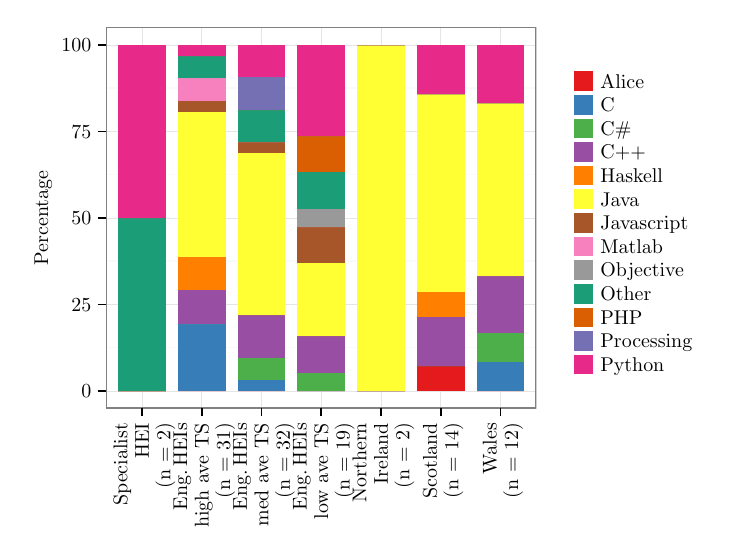
\begin{tikzpicture}[x=1pt,y=1pt]
\definecolor{fillColor}{RGB}{255,255,255}
\path[use as bounding box,fill=fillColor,fill opacity=0.00] (0,0) rectangle (252.94,180.67);
\begin{scope}
\path[clip] (  0.00,  0.00) rectangle (252.94,180.67);
\definecolor{drawColor}{RGB}{255,255,255}
\definecolor{fillColor}{RGB}{255,255,255}

\path[draw=drawColor,line width= 0.6pt,line join=round,line cap=round,fill=fillColor] (  0.00,  0.00) rectangle (252.94,180.68);
\end{scope}
\begin{scope}
\path[clip] ( 28.36, 43.19) rectangle (183.80,180.67);
\definecolor{fillColor}{RGB}{255,255,255}

\path[fill=fillColor] ( 28.36, 43.19) rectangle (183.80,180.67);
\definecolor{drawColor}{gray}{0.98}

\path[draw=drawColor,line width= 0.6pt,line join=round] ( 28.36, 65.06) --
	(183.80, 65.06);

\path[draw=drawColor,line width= 0.6pt,line join=round] ( 28.36, 96.31) --
	(183.80, 96.31);

\path[draw=drawColor,line width= 0.6pt,line join=round] ( 28.36,127.56) --
	(183.80,127.56);

\path[draw=drawColor,line width= 0.6pt,line join=round] ( 28.36,158.80) --
	(183.80,158.80);
\definecolor{drawColor}{gray}{0.90}

\path[draw=drawColor,line width= 0.2pt,line join=round] ( 28.36, 49.44) --
	(183.80, 49.44);

\path[draw=drawColor,line width= 0.2pt,line join=round] ( 28.36, 80.69) --
	(183.80, 80.69);

\path[draw=drawColor,line width= 0.2pt,line join=round] ( 28.36,111.93) --
	(183.80,111.93);

\path[draw=drawColor,line width= 0.2pt,line join=round] ( 28.36,143.18) --
	(183.80,143.18);

\path[draw=drawColor,line width= 0.2pt,line join=round] ( 28.36,174.43) --
	(183.80,174.43);

\path[draw=drawColor,line width= 0.2pt,line join=round] ( 41.31, 43.19) --
	( 41.31,180.67);

\path[draw=drawColor,line width= 0.2pt,line join=round] ( 62.90, 43.19) --
	( 62.90,180.67);

\path[draw=drawColor,line width= 0.2pt,line join=round] ( 84.49, 43.19) --
	( 84.49,180.67);

\path[draw=drawColor,line width= 0.2pt,line join=round] (106.08, 43.19) --
	(106.08,180.67);

\path[draw=drawColor,line width= 0.2pt,line join=round] (127.67, 43.19) --
	(127.67,180.67);

\path[draw=drawColor,line width= 0.2pt,line join=round] (149.26, 43.19) --
	(149.26,180.67);

\path[draw=drawColor,line width= 0.2pt,line join=round] (170.85, 43.19) --
	(170.85,180.67);
\definecolor{fillColor}{RGB}{228,26,28}

\path[fill=fillColor] ( 32.67, 49.44) rectangle ( 49.95, 49.44);
\definecolor{fillColor}{RGB}{55,126,184}

\path[fill=fillColor] ( 32.67, 49.44) rectangle ( 49.95, 49.44);
\definecolor{fillColor}{RGB}{77,175,74}

\path[fill=fillColor] ( 32.67, 49.44) rectangle ( 49.95, 49.44);
\definecolor{fillColor}{RGB}{152,78,163}

\path[fill=fillColor] ( 32.67, 49.44) rectangle ( 49.95, 49.44);
\definecolor{fillColor}{RGB}{255,127,0}

\path[fill=fillColor] ( 32.67, 49.44) rectangle ( 49.95, 49.44);
\definecolor{fillColor}{RGB}{255,255,51}

\path[fill=fillColor] ( 32.67, 49.44) rectangle ( 49.95, 49.44);
\definecolor{fillColor}{RGB}{166,86,40}

\path[fill=fillColor] ( 32.67, 49.44) rectangle ( 49.95, 49.44);
\definecolor{fillColor}{RGB}{247,129,191}

\path[fill=fillColor] ( 32.67, 49.44) rectangle ( 49.95, 49.44);
\definecolor{fillColor}{gray}{0.60}

\path[fill=fillColor] ( 32.67, 49.44) rectangle ( 49.95, 49.44);
\definecolor{fillColor}{RGB}{27,158,119}

\path[fill=fillColor] ( 32.67, 49.44) rectangle ( 49.95,111.93);
\definecolor{fillColor}{RGB}{217,95,2}

\path[fill=fillColor] ( 32.67,111.93) rectangle ( 49.95,111.93);
\definecolor{fillColor}{RGB}{117,112,179}

\path[fill=fillColor] ( 32.67,111.93) rectangle ( 49.95,111.93);
\definecolor{fillColor}{RGB}{231,41,138}

\path[fill=fillColor] ( 32.67,111.93) rectangle ( 49.95,174.43);
\definecolor{fillColor}{RGB}{228,26,28}

\path[fill=fillColor] ( 54.26, 49.44) rectangle ( 71.54, 49.44);
\definecolor{fillColor}{RGB}{55,126,184}

\path[fill=fillColor] ( 54.26, 49.44) rectangle ( 71.54, 73.63);
\definecolor{fillColor}{RGB}{77,175,74}

\path[fill=fillColor] ( 54.26, 73.63) rectangle ( 71.54, 73.63);
\definecolor{fillColor}{RGB}{152,78,163}

\path[fill=fillColor] ( 54.26, 73.63) rectangle ( 71.54, 85.73);
\definecolor{fillColor}{RGB}{255,127,0}

\path[fill=fillColor] ( 54.26, 85.73) rectangle ( 71.54, 97.82);
\definecolor{fillColor}{RGB}{255,255,51}

\path[fill=fillColor] ( 54.26, 97.82) rectangle ( 71.54,150.23);
\definecolor{fillColor}{RGB}{166,86,40}

\path[fill=fillColor] ( 54.26,150.23) rectangle ( 71.54,154.27);
\definecolor{fillColor}{RGB}{247,129,191}

\path[fill=fillColor] ( 54.26,154.27) rectangle ( 71.54,162.33);
\definecolor{fillColor}{gray}{0.60}

\path[fill=fillColor] ( 54.26,162.33) rectangle ( 71.54,162.33);
\definecolor{fillColor}{RGB}{27,158,119}

\path[fill=fillColor] ( 54.26,162.33) rectangle ( 71.54,170.39);
\definecolor{fillColor}{RGB}{217,95,2}

\path[fill=fillColor] ( 54.26,170.39) rectangle ( 71.54,170.39);
\definecolor{fillColor}{RGB}{117,112,179}

\path[fill=fillColor] ( 54.26,170.39) rectangle ( 71.54,170.39);
\definecolor{fillColor}{RGB}{231,41,138}

\path[fill=fillColor] ( 54.26,170.39) rectangle ( 71.54,174.43);
\definecolor{fillColor}{RGB}{228,26,28}

\path[fill=fillColor] ( 75.85, 49.44) rectangle ( 93.13, 49.44);
\definecolor{fillColor}{RGB}{55,126,184}

\path[fill=fillColor] ( 75.85, 49.44) rectangle ( 93.13, 53.35);
\definecolor{fillColor}{RGB}{77,175,74}

\path[fill=fillColor] ( 75.85, 53.35) rectangle ( 93.13, 61.16);
\definecolor{fillColor}{RGB}{152,78,163}

\path[fill=fillColor] ( 75.85, 61.16) rectangle ( 93.13, 76.78);
\definecolor{fillColor}{RGB}{255,127,0}

\path[fill=fillColor] ( 75.85, 76.78) rectangle ( 93.13, 76.78);
\definecolor{fillColor}{RGB}{255,255,51}

\path[fill=fillColor] ( 75.85, 76.78) rectangle ( 93.13,135.37);
\definecolor{fillColor}{RGB}{166,86,40}

\path[fill=fillColor] ( 75.85,135.37) rectangle ( 93.13,139.27);
\definecolor{fillColor}{RGB}{247,129,191}

\path[fill=fillColor] ( 75.85,139.27) rectangle ( 93.13,139.27);
\definecolor{fillColor}{gray}{0.60}

\path[fill=fillColor] ( 75.85,139.27) rectangle ( 93.13,139.27);
\definecolor{fillColor}{RGB}{27,158,119}

\path[fill=fillColor] ( 75.85,139.27) rectangle ( 93.13,150.99);
\definecolor{fillColor}{RGB}{217,95,2}

\path[fill=fillColor] ( 75.85,150.99) rectangle ( 93.13,150.99);
\definecolor{fillColor}{RGB}{117,112,179}

\path[fill=fillColor] ( 75.85,150.99) rectangle ( 93.13,162.71);
\definecolor{fillColor}{RGB}{231,41,138}

\path[fill=fillColor] ( 75.85,162.71) rectangle ( 93.13,174.43);
\definecolor{fillColor}{RGB}{228,26,28}

\path[fill=fillColor] ( 97.44, 49.44) rectangle (114.72, 49.44);
\definecolor{fillColor}{RGB}{55,126,184}

\path[fill=fillColor] ( 97.44, 49.44) rectangle (114.72, 49.44);
\definecolor{fillColor}{RGB}{77,175,74}

\path[fill=fillColor] ( 97.44, 49.44) rectangle (114.72, 56.02);
\definecolor{fillColor}{RGB}{152,78,163}

\path[fill=fillColor] ( 97.44, 56.02) rectangle (114.72, 69.17);
\definecolor{fillColor}{RGB}{255,127,0}

\path[fill=fillColor] ( 97.44, 69.17) rectangle (114.72, 69.17);
\definecolor{fillColor}{RGB}{255,255,51}

\path[fill=fillColor] ( 97.44, 69.17) rectangle (114.72, 95.49);
\definecolor{fillColor}{RGB}{166,86,40}

\path[fill=fillColor] ( 97.44, 95.49) rectangle (114.72,108.64);
\definecolor{fillColor}{RGB}{247,129,191}

\path[fill=fillColor] ( 97.44,108.64) rectangle (114.72,108.64);
\definecolor{fillColor}{gray}{0.60}

\path[fill=fillColor] ( 97.44,108.64) rectangle (114.72,115.22);
\definecolor{fillColor}{RGB}{27,158,119}

\path[fill=fillColor] ( 97.44,115.22) rectangle (114.72,128.38);
\definecolor{fillColor}{RGB}{217,95,2}

\path[fill=fillColor] ( 97.44,128.38) rectangle (114.72,141.53);
\definecolor{fillColor}{RGB}{117,112,179}

\path[fill=fillColor] ( 97.44,141.53) rectangle (114.72,141.53);
\definecolor{fillColor}{RGB}{231,41,138}

\path[fill=fillColor] ( 97.44,141.53) rectangle (114.72,174.43);
\definecolor{fillColor}{RGB}{228,26,28}

\path[fill=fillColor] (119.03, 49.44) rectangle (136.31, 49.44);
\definecolor{fillColor}{RGB}{55,126,184}

\path[fill=fillColor] (119.03, 49.44) rectangle (136.31, 49.44);
\definecolor{fillColor}{RGB}{77,175,74}

\path[fill=fillColor] (119.03, 49.44) rectangle (136.31, 49.44);
\definecolor{fillColor}{RGB}{152,78,163}

\path[fill=fillColor] (119.03, 49.44) rectangle (136.31, 49.44);
\definecolor{fillColor}{RGB}{255,127,0}

\path[fill=fillColor] (119.03, 49.44) rectangle (136.31, 49.44);
\definecolor{fillColor}{RGB}{255,255,51}

\path[fill=fillColor] (119.03, 49.44) rectangle (136.31,174.43);
\definecolor{fillColor}{RGB}{166,86,40}

\path[fill=fillColor] (119.03,174.43) rectangle (136.31,174.43);
\definecolor{fillColor}{RGB}{247,129,191}

\path[fill=fillColor] (119.03,174.43) rectangle (136.31,174.43);
\definecolor{fillColor}{gray}{0.60}

\path[fill=fillColor] (119.03,174.43) rectangle (136.31,174.43);
\definecolor{fillColor}{RGB}{27,158,119}

\path[fill=fillColor] (119.03,174.43) rectangle (136.31,174.43);
\definecolor{fillColor}{RGB}{217,95,2}

\path[fill=fillColor] (119.03,174.43) rectangle (136.31,174.43);
\definecolor{fillColor}{RGB}{117,112,179}

\path[fill=fillColor] (119.03,174.43) rectangle (136.31,174.43);
\definecolor{fillColor}{RGB}{231,41,138}

\path[fill=fillColor] (119.03,174.43) rectangle (136.31,174.43);
\definecolor{fillColor}{RGB}{228,26,28}

\path[fill=fillColor] (140.62, 49.44) rectangle (157.90, 58.37);
\definecolor{fillColor}{RGB}{55,126,184}

\path[fill=fillColor] (140.62, 58.37) rectangle (157.90, 58.37);
\definecolor{fillColor}{RGB}{77,175,74}

\path[fill=fillColor] (140.62, 58.37) rectangle (157.90, 58.37);
\definecolor{fillColor}{RGB}{152,78,163}

\path[fill=fillColor] (140.62, 58.37) rectangle (157.90, 76.22);
\definecolor{fillColor}{RGB}{255,127,0}

\path[fill=fillColor] (140.62, 76.22) rectangle (157.90, 85.15);
\definecolor{fillColor}{RGB}{255,255,51}

\path[fill=fillColor] (140.62, 85.15) rectangle (157.90,156.57);
\definecolor{fillColor}{RGB}{166,86,40}

\path[fill=fillColor] (140.62,156.57) rectangle (157.90,156.57);
\definecolor{fillColor}{RGB}{247,129,191}

\path[fill=fillColor] (140.62,156.57) rectangle (157.90,156.57);
\definecolor{fillColor}{gray}{0.60}

\path[fill=fillColor] (140.62,156.57) rectangle (157.90,156.57);
\definecolor{fillColor}{RGB}{27,158,119}

\path[fill=fillColor] (140.62,156.57) rectangle (157.90,156.57);
\definecolor{fillColor}{RGB}{217,95,2}

\path[fill=fillColor] (140.62,156.57) rectangle (157.90,156.57);
\definecolor{fillColor}{RGB}{117,112,179}

\path[fill=fillColor] (140.62,156.57) rectangle (157.90,156.57);
\definecolor{fillColor}{RGB}{231,41,138}

\path[fill=fillColor] (140.62,156.57) rectangle (157.90,174.43);
\definecolor{fillColor}{RGB}{228,26,28}

\path[fill=fillColor] (162.21, 49.44) rectangle (179.49, 49.44);
\definecolor{fillColor}{RGB}{55,126,184}

\path[fill=fillColor] (162.21, 49.44) rectangle (179.49, 59.86);
\definecolor{fillColor}{RGB}{77,175,74}

\path[fill=fillColor] (162.21, 59.86) rectangle (179.49, 70.27);
\definecolor{fillColor}{RGB}{152,78,163}

\path[fill=fillColor] (162.21, 70.27) rectangle (179.49, 91.10);
\definecolor{fillColor}{RGB}{255,127,0}

\path[fill=fillColor] (162.21, 91.10) rectangle (179.49, 91.10);
\definecolor{fillColor}{RGB}{255,255,51}

\path[fill=fillColor] (162.21, 91.10) rectangle (179.49,153.59);
\definecolor{fillColor}{RGB}{166,86,40}

\path[fill=fillColor] (162.21,153.59) rectangle (179.49,153.59);
\definecolor{fillColor}{RGB}{247,129,191}

\path[fill=fillColor] (162.21,153.59) rectangle (179.49,153.59);
\definecolor{fillColor}{gray}{0.60}

\path[fill=fillColor] (162.21,153.59) rectangle (179.49,153.59);
\definecolor{fillColor}{RGB}{27,158,119}

\path[fill=fillColor] (162.21,153.59) rectangle (179.49,153.59);
\definecolor{fillColor}{RGB}{217,95,2}

\path[fill=fillColor] (162.21,153.59) rectangle (179.49,153.59);
\definecolor{fillColor}{RGB}{117,112,179}

\path[fill=fillColor] (162.21,153.59) rectangle (179.49,153.59);
\definecolor{fillColor}{RGB}{231,41,138}

\path[fill=fillColor] (162.21,153.59) rectangle (179.49,174.43);
\definecolor{drawColor}{gray}{0.50}

\path[draw=drawColor,line width= 0.6pt,line join=round,line cap=round] ( 28.36, 43.19) rectangle (183.80,180.67);
\end{scope}
\begin{scope}
\path[clip] (  0.00,  0.00) rectangle (252.94,180.67);
\definecolor{drawColor}{RGB}{0,0,0}

\node[text=drawColor,anchor=base east,inner sep=0pt, outer sep=0pt, scale=  0.72] at ( 22.96, 46.96) {0};

\node[text=drawColor,anchor=base east,inner sep=0pt, outer sep=0pt, scale=  0.72] at ( 22.96, 78.21) {25};

\node[text=drawColor,anchor=base east,inner sep=0pt, outer sep=0pt, scale=  0.72] at ( 22.96,109.45) {50};

\node[text=drawColor,anchor=base east,inner sep=0pt, outer sep=0pt, scale=  0.72] at ( 22.96,140.70) {75};

\node[text=drawColor,anchor=base east,inner sep=0pt, outer sep=0pt, scale=  0.72] at ( 22.96,171.95) {100};
\end{scope}
\begin{scope}
\path[clip] (  0.00,  0.00) rectangle (252.94,180.67);
\definecolor{drawColor}{RGB}{0,0,0}

\path[draw=drawColor,line width= 0.6pt,line join=round] ( 25.36, 49.44) --
	( 28.36, 49.44);

\path[draw=drawColor,line width= 0.6pt,line join=round] ( 25.36, 80.69) --
	( 28.36, 80.69);

\path[draw=drawColor,line width= 0.6pt,line join=round] ( 25.36,111.93) --
	( 28.36,111.93);

\path[draw=drawColor,line width= 0.6pt,line join=round] ( 25.36,143.18) --
	( 28.36,143.18);

\path[draw=drawColor,line width= 0.6pt,line join=round] ( 25.36,174.43) --
	( 28.36,174.43);
\end{scope}
\begin{scope}
\path[clip] (  0.00,  0.00) rectangle (252.94,180.67);
\definecolor{drawColor}{RGB}{0,0,0}

\path[draw=drawColor,line width= 0.6pt,line join=round] ( 41.31, 40.19) --
	( 41.31, 43.19);

\path[draw=drawColor,line width= 0.6pt,line join=round] ( 62.90, 40.19) --
	( 62.90, 43.19);

\path[draw=drawColor,line width= 0.6pt,line join=round] ( 84.49, 40.19) --
	( 84.49, 43.19);

\path[draw=drawColor,line width= 0.6pt,line join=round] (106.08, 40.19) --
	(106.08, 43.19);

\path[draw=drawColor,line width= 0.6pt,line join=round] (127.67, 40.19) --
	(127.67, 43.19);

\path[draw=drawColor,line width= 0.6pt,line join=round] (149.26, 40.19) --
	(149.26, 43.19);

\path[draw=drawColor,line width= 0.6pt,line join=round] (170.85, 40.19) --
	(170.85, 43.19);
\end{scope}
\begin{scope}
\path[clip] (  0.00,  0.00) rectangle (252.94,180.67);
\definecolor{drawColor}{RGB}{0,0,0}

\node[text=drawColor,rotate= 90.00,anchor=base east,inner sep=0pt, outer sep=0pt, scale=  0.72] at ( 36.01, 37.79) {Specialist};

\node[text=drawColor,rotate= 90.00,anchor=base east,inner sep=0pt, outer sep=0pt, scale=  0.72] at ( 43.79, 37.79) {HEI};

\node[text=drawColor,rotate= 90.00,anchor=base east,inner sep=0pt, outer sep=0pt, scale=  0.72] at ( 51.57, 37.79) {(n = 2)};

\node[text=drawColor,rotate= 90.00,anchor=base east,inner sep=0pt, outer sep=0pt, scale=  0.72] at ( 57.60, 37.79) {Eng.\,HEIs};

\node[text=drawColor,rotate= 90.00,anchor=base east,inner sep=0pt, outer sep=0pt, scale=  0.72] at ( 65.38, 37.79) {high ave TS};

\node[text=drawColor,rotate= 90.00,anchor=base east,inner sep=0pt, outer sep=0pt, scale=  0.72] at ( 73.16, 37.79) {(n = 31)};

\node[text=drawColor,rotate= 90.00,anchor=base east,inner sep=0pt, outer sep=0pt, scale=  0.72] at ( 79.19, 37.79) {Eng.\,HEIs};

\node[text=drawColor,rotate= 90.00,anchor=base east,inner sep=0pt, outer sep=0pt, scale=  0.72] at ( 86.97, 37.79) {med ave TS};

\node[text=drawColor,rotate= 90.00,anchor=base east,inner sep=0pt, outer sep=0pt, scale=  0.72] at ( 94.75, 37.79) {(n = 32)};

\node[text=drawColor,rotate= 90.00,anchor=base east,inner sep=0pt, outer sep=0pt, scale=  0.72] at (100.78, 37.79) {Eng.\,HEIs};

\node[text=drawColor,rotate= 90.00,anchor=base east,inner sep=0pt, outer sep=0pt, scale=  0.72] at (108.56, 37.79) {low ave TS};

\node[text=drawColor,rotate= 90.00,anchor=base east,inner sep=0pt, outer sep=0pt, scale=  0.72] at (116.33, 37.79) {(n = 19)};

\node[text=drawColor,rotate= 90.00,anchor=base east,inner sep=0pt, outer sep=0pt, scale=  0.72] at (122.37, 37.79) {Northern};

\node[text=drawColor,rotate= 90.00,anchor=base east,inner sep=0pt, outer sep=0pt, scale=  0.72] at (130.15, 37.79) {Ireland};

\node[text=drawColor,rotate= 90.00,anchor=base east,inner sep=0pt, outer sep=0pt, scale=  0.72] at (137.92, 37.79) {(n = 2)};

\node[text=drawColor,rotate= 90.00,anchor=base east,inner sep=0pt, outer sep=0pt, scale=  0.72] at (147.85, 37.79) {Scotland};

\node[text=drawColor,rotate= 90.00,anchor=base east,inner sep=0pt, outer sep=0pt, scale=  0.72] at (155.63, 37.79) {(n = 14)};

\node[text=drawColor,rotate= 90.00,anchor=base east,inner sep=0pt, outer sep=0pt, scale=  0.72] at (169.44, 37.79) {Wales};

\node[text=drawColor,rotate= 90.00,anchor=base east,inner sep=0pt, outer sep=0pt, scale=  0.72] at (177.22, 37.79) {(n = 12)};
\end{scope}
\begin{scope}
\path[clip] (  0.00,  0.00) rectangle (252.94,180.67);
\definecolor{drawColor}{RGB}{0,0,0}

\node[text=drawColor,rotate= 90.00,anchor=base,inner sep=0pt, outer sep=0pt, scale=  0.72] at (  7.36,111.93) {Percentage};
\end{scope}
\begin{scope}
\path[clip] (  0.00,  0.00) rectangle (252.94,180.67);
\definecolor{fillColor}{RGB}{255,255,255}

\path[fill=fillColor] (192.34, 50.38) rectangle (244.41,173.49);
\end{scope}
\begin{scope}
\path[clip] (  0.00,  0.00) rectangle (252.94,180.67);
\definecolor{fillColor}{RGB}{228,26,28}

\path[fill=fillColor] (197.32,157.78) rectangle (204.43,164.90);
\end{scope}
\begin{scope}
\path[clip] (  0.00,  0.00) rectangle (252.94,180.67);
\definecolor{fillColor}{RGB}{55,126,184}

\path[fill=fillColor] (197.32,149.25) rectangle (204.43,156.36);
\end{scope}
\begin{scope}
\path[clip] (  0.00,  0.00) rectangle (252.94,180.67);
\definecolor{fillColor}{RGB}{77,175,74}

\path[fill=fillColor] (197.32,140.71) rectangle (204.43,147.83);
\end{scope}
\begin{scope}
\path[clip] (  0.00,  0.00) rectangle (252.94,180.67);
\definecolor{fillColor}{RGB}{152,78,163}

\path[fill=fillColor] (197.32,132.18) rectangle (204.43,139.29);
\end{scope}
\begin{scope}
\path[clip] (  0.00,  0.00) rectangle (252.94,180.67);
\definecolor{fillColor}{RGB}{255,127,0}

\path[fill=fillColor] (197.32,123.64) rectangle (204.43,130.75);
\end{scope}
\begin{scope}
\path[clip] (  0.00,  0.00) rectangle (252.94,180.67);
\definecolor{fillColor}{RGB}{255,255,51}

\path[fill=fillColor] (197.32,115.11) rectangle (204.43,122.22);
\end{scope}
\begin{scope}
\path[clip] (  0.00,  0.00) rectangle (252.94,180.67);
\definecolor{fillColor}{RGB}{166,86,40}

\path[fill=fillColor] (197.32,106.57) rectangle (204.43,113.68);
\end{scope}
\begin{scope}
\path[clip] (  0.00,  0.00) rectangle (252.94,180.67);
\definecolor{fillColor}{RGB}{247,129,191}

\path[fill=fillColor] (197.32, 98.03) rectangle (204.43,105.15);
\end{scope}
\begin{scope}
\path[clip] (  0.00,  0.00) rectangle (252.94,180.67);
\definecolor{fillColor}{gray}{0.60}

\path[fill=fillColor] (197.32, 89.50) rectangle (204.43, 96.61);
\end{scope}
\begin{scope}
\path[clip] (  0.00,  0.00) rectangle (252.94,180.67);
\definecolor{fillColor}{RGB}{27,158,119}

\path[fill=fillColor] (197.32, 80.96) rectangle (204.43, 88.08);
\end{scope}
\begin{scope}
\path[clip] (  0.00,  0.00) rectangle (252.94,180.67);
\definecolor{fillColor}{RGB}{217,95,2}

\path[fill=fillColor] (197.32, 72.43) rectangle (204.43, 79.54);
\end{scope}
\begin{scope}
\path[clip] (  0.00,  0.00) rectangle (252.94,180.67);
\definecolor{fillColor}{RGB}{117,112,179}

\path[fill=fillColor] (197.32, 63.89) rectangle (204.43, 71.00);
\end{scope}
\begin{scope}
\path[clip] (  0.00,  0.00) rectangle (252.94,180.67);
\definecolor{fillColor}{RGB}{231,41,138}

\path[fill=fillColor] (197.32, 55.35) rectangle (204.43, 62.47);
\end{scope}
\begin{scope}
\path[clip] (  0.00,  0.00) rectangle (252.94,180.67);
\definecolor{drawColor}{RGB}{0,0,0}

\node[text=drawColor,anchor=base west,inner sep=0pt, outer sep=0pt, scale=  0.72] at (206.95,158.86) {Alice};
\end{scope}
\begin{scope}
\path[clip] (  0.00,  0.00) rectangle (252.94,180.67);
\definecolor{drawColor}{RGB}{0,0,0}

\node[text=drawColor,anchor=base west,inner sep=0pt, outer sep=0pt, scale=  0.72] at (206.95,150.33) {C};
\end{scope}
\begin{scope}
\path[clip] (  0.00,  0.00) rectangle (252.94,180.67);
\definecolor{drawColor}{RGB}{0,0,0}

\node[text=drawColor,anchor=base west,inner sep=0pt, outer sep=0pt, scale=  0.72] at (206.95,141.79) {C\#};
\end{scope}
\begin{scope}
\path[clip] (  0.00,  0.00) rectangle (252.94,180.67);
\definecolor{drawColor}{RGB}{0,0,0}

\node[text=drawColor,anchor=base west,inner sep=0pt, outer sep=0pt, scale=  0.72] at (206.95,133.25) {C++};
\end{scope}
\begin{scope}
\path[clip] (  0.00,  0.00) rectangle (252.94,180.67);
\definecolor{drawColor}{RGB}{0,0,0}

\node[text=drawColor,anchor=base west,inner sep=0pt, outer sep=0pt, scale=  0.72] at (206.95,124.72) {Haskell};
\end{scope}
\begin{scope}
\path[clip] (  0.00,  0.00) rectangle (252.94,180.67);
\definecolor{drawColor}{RGB}{0,0,0}

\node[text=drawColor,anchor=base west,inner sep=0pt, outer sep=0pt, scale=  0.72] at (206.95,116.18) {Java};
\end{scope}
\begin{scope}
\path[clip] (  0.00,  0.00) rectangle (252.94,180.67);
\definecolor{drawColor}{RGB}{0,0,0}

\node[text=drawColor,anchor=base west,inner sep=0pt, outer sep=0pt, scale=  0.72] at (206.95,107.65) {Javascript};
\end{scope}
\begin{scope}
\path[clip] (  0.00,  0.00) rectangle (252.94,180.67);
\definecolor{drawColor}{RGB}{0,0,0}

\node[text=drawColor,anchor=base west,inner sep=0pt, outer sep=0pt, scale=  0.72] at (206.95, 99.11) {Matlab};
\end{scope}
\begin{scope}
\path[clip] (  0.00,  0.00) rectangle (252.94,180.67);
\definecolor{drawColor}{RGB}{0,0,0}

\node[text=drawColor,anchor=base west,inner sep=0pt, outer sep=0pt, scale=  0.72] at (206.95, 90.58) {Objective};
\end{scope}
\begin{scope}
\path[clip] (  0.00,  0.00) rectangle (252.94,180.67);
\definecolor{drawColor}{RGB}{0,0,0}

\node[text=drawColor,anchor=base west,inner sep=0pt, outer sep=0pt, scale=  0.72] at (206.95, 82.04) {Other};
\end{scope}
\begin{scope}
\path[clip] (  0.00,  0.00) rectangle (252.94,180.67);
\definecolor{drawColor}{RGB}{0,0,0}

\node[text=drawColor,anchor=base west,inner sep=0pt, outer sep=0pt, scale=  0.72] at (206.95, 73.50) {PHP};
\end{scope}
\begin{scope}
\path[clip] (  0.00,  0.00) rectangle (252.94,180.67);
\definecolor{drawColor}{RGB}{0,0,0}

\node[text=drawColor,anchor=base west,inner sep=0pt, outer sep=0pt, scale=  0.72] at (206.95, 64.97) {Processing};
\end{scope}
\begin{scope}
\path[clip] (  0.00,  0.00) rectangle (252.94,180.67);
\definecolor{drawColor}{RGB}{0,0,0}

\node[text=drawColor,anchor=base west,inner sep=0pt, outer sep=0pt, scale=  0.72] at (206.95, 56.43) {Python};
\end{scope}
\end{tikzpicture}
